\section{The result and the gap it closes}
\label{sec:main}

The source program has a substantial finite-field strand: spanning estimates,
symplectic frames, compressed observations, and the extent to which partial
linear information reveals an underlying alternating form. The present paper
continues that strand. Its connection to the GRH project is methodological and
explicit; no assertion about zeros of an $L$-function is used in any proof.

The immediate predecessors \cite{hidden,critical} already established the
sample threshold and the distribution of the candidate space's dimension.
The remaining question is more precise: \emph{how many of those linear
candidates are actually nondegenerate, and how much does that information
improve testing and recovery?} Two spaces of the same dimension can have very
different answers. Our main theorem determines this missing distribution.

\subsection{The experiment}

Fix a prime power $q$ and let $n\ge4$ be even. Put
\[
 V=\F^n,\qquad E=\Alt(V),\qquad
 D=\binom n2,\qquad d=D-1.
\]
Here an alternating form is a bilinear form $H$ with $H(v,v)=0$ for every
$v$. This definition also applies in characteristic two. Nondegeneracy means
that $H(v,w)=0$ for every $w$ forces $v=0$. Forms differing by a nonzero scalar
are identified; a projective form is such an equivalence class.

Under the \emph{null law} $Q_{n,t}$ we observe independent uniform
two-dimensional subspaces $\Pi_1,\ldots,\Pi_t$ of $V$.
Under the \emph{planted law} $P_{n,t}$ we first choose a uniform nondegenerate
projective form $[H]$, and then independently choose each $\Pi_i$ uniformly
among the $H$-isotropic two-planes. Thus $H$ is chosen once and is common to
every observation. Define
\begin{align}
 N&=\{G\in E:G|_{\Pi_i\times\Pi_i}=0\text{ for all }i\},
 &K&=\dim N,\label{eq:candidates}\\
 Z&=\#\{[G]\in\mathbb P(N):G\text{ is nondegenerate}\}.
 \label{eq:Z}
\end{align}
The entire space $N$ is found by solving $t$ homogeneous linear equations in
$D$ unknowns. Under the planted law, $Z\ge1$ because $[H]$ is a candidate.

\subsection{The explicit critical distribution}

Use the constants and probability masses
\begin{gather}
 g_j=\prod_{i=1}^j(1-q^{-i}),\qquad
 g_\infty=\prod_{i\ge1}(1-q^{-i}),\qquad
 \omega_q=\prod_{i\ge1}(1-q^{-(2i-1)}),\label{eq:products}\\
 c_q=\frac{\omega_q}{1-q^{-1}},\qquad
 m_k=\frac{q^k-1}{q-1},\qquad
 \lambda_a=c_q q^{-a},\label{eq:constants}\\
 \pi_b(k)=\frac{g_\infty q^{-k(k+b)}}{g_k g_{k+b}}\quad
 (k\ge\max(0,-b)),\label{eq:pi}
\end{gather}
and set $\pi_b(k)=0$ elsewhere. The law $\pi_b$ is the classical limiting
kernel dimension of a uniform $(D+b)\times D$ matrix over $\F$ as
$D\to\infty$ \cite{fulman}. It is not a new marginal distribution.

\begin{theorem}[The complete critical experiment]
\label{thm:main}
Fix $q$ and an integer $a$, and set $t=d+a$. As even $n\to\infty$, the joint
law of $(K,Z)$ converges in total variation as follows.
\begin{enumerate}
\item Under $Q_{n,t}$, draw
\[
 K\sim\pi_{a-1},\qquad Z\mid K=k\sim\Bin(m_k,\omega_q).
 \tag{Q}\label{eq:Q-limit}
\]
In particular $Z=0$ when $K=0$.
\item Under $P_{n,t}$, draw
\[
 J\sim\pi_a,\qquad K=1+J,\qquad
 Z\mid K=k\sim1+\Bin(m_k-1,\omega_q).
 \tag{P}\label{eq:P-limit}
\]
\item If $\mathsf Q_a$ denotes the joint law in \eqref{eq:Q-limit}, the law
in \eqref{eq:P-limit} satisfies
\begin{equation}
 \mathsf P_a(k,z)=\frac{z}{\lambda_a}\mathsf Q_a(k,z).
 \label{eq:sizebias}
\end{equation}
The statistic $Z$ determines the exact finite-sample likelihood ratio, so
these formulas determine the limiting optimum over all tests of the complete
observations.
\end{enumerate}
\end{theorem}

The binomial statement is conditional on a \emph{fixed finite} dimension.
It does not assert finite-$n$ independence, or independence for a number of
forms growing with $n$. The candidate dimension remains random in the limit;
averaging that randomness is essential.

\begin{corollary}[Optimal testing and recovery curves]
\label{cor:curves}
With $(K,Z)\sim\mathsf Q_a$, define
\begin{align}
 T_q(a)&=\frac12\E\left|\frac{Z}{\lambda_a}-1\right|,
 \label{eq:T}\\
 R_q(a)&=\frac1{\lambda_a}
 \sum_{k\ge0}\pi_{a-1}(k)\bigl[1-(1-\omega_q)^{m_k}\bigr],
 \label{eq:R}\\
 U_q(a)&=\sum_{k\ge1}\pi_a(k-1)(1-\omega_q)^{m_k-1}.
 \label{eq:U}
\end{align}
Then $\TV(P_{n,d+a},Q_{n,d+a})\to T_q(a)$; the optimal probability of
recovering the hidden projective form tends to $R_q(a)$; and, under the
planted law, the probability of a unique compatible nondegenerate projective
form tends to $U_q(a)$.
For $a\ge0$, the exact finite-sample optimal test declares the planted law
precisely when $Z>0$, and
\begin{equation}
 T_q(a)=\sum_{k\ge0}\pi_{a-1}(k)(1-\omega_q)^{m_k},\qquad
 R_q(a)=\frac{1-T_q(a)}{\lambda_a}.
 \label{eq:nonnegative}
\end{equation}
The best equal-prior testing success probability tends to $(1+T_q(a))/2$.
\end{corollary}

\subsection{What is gained}

For comparison, the previously known dimension-only testing distance and
linear uniqueness probability are
\begin{align}
 T_q^{\rm dim}(a)&=
 \begin{cases}
 q^{a-1}g_\infty/g_{1-a},&a\le0,\\
 g_\infty/g_{a-1},&a\ge1,
 \end{cases}\label{eq:dimension-curve}\\
 F_q(a)&=\begin{cases}g_\infty/g_a,&a\ge0,\\0,&a<0.\end{cases}
 \label{eq:linear-curve}
\end{align}
We rederive these comparisons below. The new result gives the strict
inequalities
\begin{equation}
 T_q(a)>T_q^{\rm dim}(a),\qquad
 R_q(a)>U_q(a)>F_q(a)\quad(a\in\mathbb Z).
 \label{eq:strict-gain}
\end{equation}
The second inequality is interpreted with $F_q(a)=0$ for negative offsets.
Thus uniqueness among nondegenerate forms can occur even before linear
uniqueness is possible.

For $q=2$ the central offset $a=0$ gives
\[
 T_2(0)=0.411496025791\ldots,\qquad
 T_2^{\rm dim}(0)=0.288788095087\ldots,
\]
and
\[
 R_2(0)=0.701564718009\ldots,\quad
 U_2(0)=0.488389858129\ldots,\quad
 F_2(0)=0.288788095087\ldots.
\]
At $a=-1$, optimal recovery still succeeds with limiting probability
$0.503310957568\ldots$, although a one-dimensional linear candidate space is
impossible. These are limiting probabilities, not finite-size guarantees.

\begin{figure}[htbp]
 \centering
 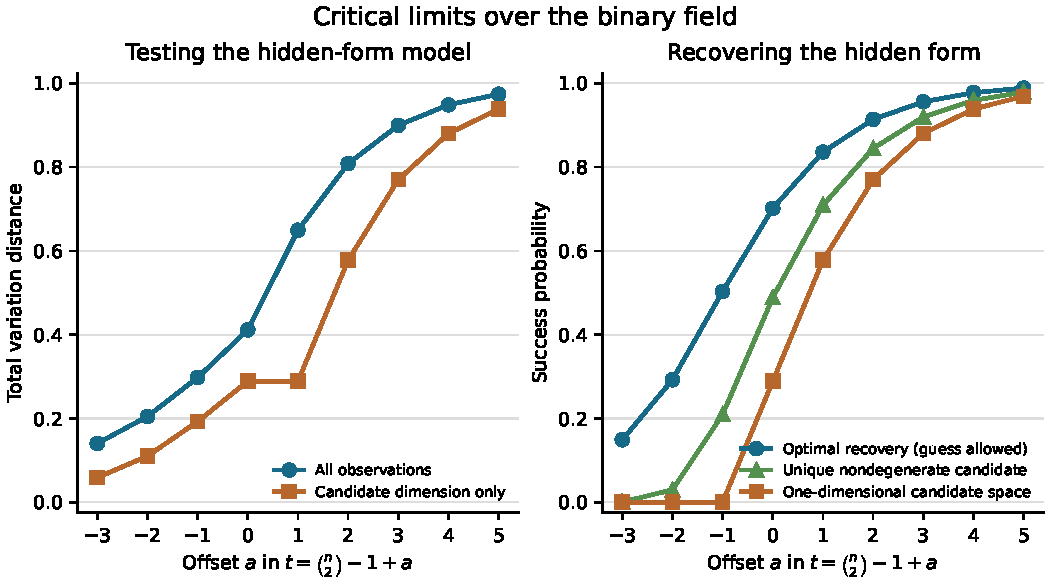
\includegraphics[width=\textwidth]{figures/critical_profiles.pdf}
 \caption{The proved binary-field critical curves. The horizontal variable
 is the integer offset from $d=\binom n2-1$. Lines connect integer evaluations
 for readability; no continuous-offset interpolation is asserted.}
 \label{fig:profiles}
\end{figure}

\subsection{Two independent mathematical advances}

The first new ingredient, \cref{ker:theorem}, replaces the full law of $N$ by
that of the kernel of independent uniform linear equations. Its conclusion
concerns the actual subspace, including its position, and is stronger than a
nullity law. The rows in the observation model are decomposable bivectors,
with extensive dependence among their entries.

The second ingredient, \cref{thm:pencil}, states that the invertibility
indicators of all distinct projective combinations of a fixed family of large
random alternating matrices become independent. As a standalone consequence,
every prescribed pattern of singular and nonsingular projective combinations
has a positive limiting probability. Combining these ingredients with the
exact likelihood gives \cref{thm:main}.

There is also an algorithmic consequence: in the fixed critical window the
exact optimal test and a Bayes optimal recovery rule can be implemented with
$O_{q,a}(n^6)$ expected field operations under either experiment. This is an
expected bound; the candidate enumeration can be exponential on exceptional
inputs. See \cref{prop:algorithm}.
